\documentclass{IEEEtran}
\usepackage{cite}
\usepackage{amsmath,amssymb,amsfonts}
\usepackage{algorithmic}
\usepackage{graphicx}
\usepackage{pgfplots}
\usepackage{tikz}
\usepackage{textcomp}
\usepackage{booktabs}
\usepackage{listings}
\usepackage{xcolor} % for setting colors
\definecolor{vblue}{RGB}{49,49,255}
\definecolor{vgreen}{RGB}{104,180,104}

\usepackage {tikz}
\usetikzlibrary {positioning}
%\usepackage {xcolor}
\definecolor {processblue}{cmyk}{0.96,0,0,0}

\definecolor{light-gray}{gray}{0.95} %the shade of grey that stack exchange uses
% set the default code style
\lstset{
	basicstyle=\ttfamily,  
	backgroundcolor=\color{light-gray}
}
 \lstdefinestyle{cpp}{
 	language=C++,
 	basicstyle=\small\ttfamily,
 	keywordstyle=\color{vblue},
 	identifierstyle=\color{black},
 	commentstyle=\color{vgreen},
 	numberstyle=\tiny\color{black},
 	numbersep=10pt,
 	tabsize=4,
 	moredelim=*[s][\colorIndex]{[}{]},
 	literate=*{:}{:}1
 }

\def\BibTeX{{\rm B\kern-.05em{\sc i\kern-.025em b}\kern-.08em
		T\kern-.1667em\lower.7ex\hbox{E}\kern-.125emX}}
\begin{document}
\title{Parallel Congruence Closure SAT solver}
\author{Enrico Martini, VR445204}
\maketitle
\begin{abstract}
 In this report is presented a parallel implementation of a congruence closure algorithm for deduction in ground equational theories, able to solve a set of clauses in the quantifiers free fragment of first order logic, based on equality among variables, constants, function applications, recursive data structures with their elements and elements of arrays.
\end{abstract}
\section{Introduction}
The first theory considered is the class of SMT problems is called EUF (Equality with Uninterpreted Functions), containing atoms that are equalities between terms built over uninterpreted function symbols. EUF (i.e., SAT modulo the theory of congruences) is important in applications such as the verification of pipelined processors, where, if the control is verified, the concrete data operations can be abstracted by uninterpreted function symbols.\cite{NIEUWENHUIS2007557} It is the most important theory because its congruence closure algorithm is the core of the entire solver. The implemented algorithm also integrates the theory of lists $\mathcal{T}_{cons}$. 
\section{Methodology}


\subsection{Algorithm}
The most interesting feature of this implementation is the organization of the information within the data structures, shaped to be efficient.
\paragraph{Node} 
The design of the \verb|Node| structure was mainly inspired by the interpretation of  \textit{'The Calculus of Computation'}\cite{10.5555/1324777}, which describes a resolution procedure for the above mentioned theories. The \verb|id| field holds the node’s unique identification number; the \verb|fn| field holds the constant or function symbol and the \verb|args| field holds a list of identification numbers representing the function arguments. The \verb|find| field holds the identification number of another node (possibly itself) in its congruence class. Following a chain of \verb|find| references leads to the representative of the congruence class. A representative node’s find field points to the node itself. If a node is the representative for its congruence class, then its \verb|ccpar| (for congruence closure parents) field stores the set of all parents of all nodes in its congruence class.
\begin{lstlisting}[style=cpp]
class Node{
private:
	std::string 		fn;                  
	int			 		id;                
	std::vector<int> 	args; 
	int			 		find;              
	std::vector<int>	ccpar;
};
\end{lstlisting}

\paragraph{Clause} 
The \verb|Clause| class is used to save nodes while maintaining the given input relationship. It allows two nodes to be related but has no methods to compare them, as they are used in another class.
\begin{lstlisting}[style=cpp]
class Clause{
private:
	Node n1;
	Node n2;
	bool is_equal;
}
\end{lstlisting}

\paragraph{Formula}
The \verb|Formula| class contains a single vector of clauses. This structure is the exact transposition of the given input string to be resolved. Once the formula is created the initial string can be discarded because all relevant information has been saved.
\begin{lstlisting}[style=cpp]
class Formula{
private:
	std::vector<Clause> v_set;
};
\end{lstlisting}

\paragraph{Sat}
The \verb|Sat| class acts as a wrapper for the entire program. It contains methods for interfacing with the solver and methods for string parsing. Inside it is saved the initial translated formula and the set of nodes on which the congruence closure will be performed. There are also two index vectors, useful for checking the type of elements. In this case, since the array theory is also included, it has been mandatory to introduce a type checking system that is able to detect any errors in the provided string, such as the comparison between two arrays that is not possible to do in the array theory without extensionality, due to the decision procedure for T$_A$-satisfiability of quantifier-free $\sum_A$-formula F is based on a reduction to T$_E$-satisfiability via applications of the (read-over-write) axioms. 

\begin{lstlisting}[style=cpp]
class Sat{
private:
	Formula 			f;
	std::vector<Node> 	n_set;
	std::vector<int> 	atoms;
	std::vector<int> 	arrays;

	bool	is_legal();
	int 	transform_node(std::string n);
	void 	initialize_DAG(std::string input);
	bool 	classic_congruence_closure();
	bool 	list_congruence_closure();
	std::vector<std::string> 
			split_arguments(std::string s);

	int 			 FIND(int index);
	void 			 UNION(int i1, int i2);
	std::vector<int> CCPAR(int index);
	bool 			 CONGRUENT(int i1, int i2);
	void 			 MERGE(int i1, int i2);

public:
	static std::vector<std::string> 
					split(std::string s);
	static bool well_formed(std::string s);
	static bool solve(std::string s);
	static std::vector<std::string> 
			detect_store(std::string input);
};
\end{lstlisting}

















\subsection{Equality theory congruence closure example}
\begin{align*}
	\mathcal{F} : x = y \land f(x) \ne f(y)
\end{align*}

\begin{lstlisting}
x=y&f(x)!=f(y)
\end{lstlisting}

\begin {center}
\resizebox{3.5cm}{!}{
\begin {tikzpicture}[-latex ,auto ,node distance =2 cm and 2cm ,on grid ,
semithick ,
state/.style ={ circle ,top color =white , bottom color = white ,
	draw,black , text=black , minimum width =0.5 cm}]
\node[state] (N0) {0 : x};
\node[state] (N1) [right=of N0]{1 : y};
\node[state] (N2) [above =of N0]{2 : f};
\node[state] (N3) [above right=of N0] {3 : f};
\path (N2) edge [above] node[left] {} (N0);
\path (N3) edge [above] node[left] {} (N1);
\end{tikzpicture}
}
\end{center}

\begin{lstlisting}
node		find		ccpar
________________________________________
0x		0		2
1y		1		3
2f->0		2		-
3f->1		3		-
\end{lstlisting}

\begin{lstlisting}
MERGE 0 1
UNION 0 1
MERGE 2 3 ?
CONGRUENT 2 3 = 1
\end{lstlisting}


\begin {center}
\resizebox{3.5cm}{!}{
	\begin {tikzpicture}[-latex ,auto ,node distance =2 cm and 2cm ,on grid ,
	semithick ,
	state/.style ={ circle ,top color =white , bottom color = white ,
		draw,black , text=black , minimum width =0.5 cm}]
	\node[state] (N0) {0 : x};
	\node[state] (N1) [right=of N0]{1 : y};
	\node[state] (N2) [above =of N0]{2 : f};
	\node[state] (N3) [above right=of N0] {3 : f};
	\path (N2) edge [above] node[left] {} (N0);
	\path (N3) edge [above] node[left] {} (N0);
	\path (N0) edge[,-,densely dotted] [above] node[left] {} (N1);
\end{tikzpicture}
}
\end{center}

\begin{lstlisting}
node		find		ccpar
________________________________________
0x		0		23
1y		0		-
2f->0		2		-
3f->1		3		-
\end{lstlisting}

\begin{lstlisting}
MERGE 2 3
UNION 2 3
\end{lstlisting}

\begin {center}
\resizebox{3.5cm}{!}{
	\begin {tikzpicture}[-latex ,auto ,node distance =2 cm and 2cm ,on grid ,
	semithick ,
	state/.style ={ circle ,top color =white , bottom color = white ,
		draw,black , text=black , minimum width =0.5 cm}]
	\node[state] (N0) {0 : x};
	\node[state] (N1) [right=of N0]{1 : y};
	\node[state] (N2) [above =of N0]{2 : f};
	\node[state] (N3) [above right=of N0] {3 : f};
	\path (N2) edge [above] node[left] {} (N0);
	\path (N3) edge [above] node[left] {} (N0);
	\path (N0) edge[,-,densely dotted] [above] node[left] {} (N1);		\path (N2) edge[,-,densely dotted] [above] node[left] {} (N3);
\end{tikzpicture}
}
\end{center}

\begin{lstlisting}
node		find		ccpar
________________________________________
0x		0		23
1y		0		-
2f->0		2		-
3f->1		2		-
\end{lstlisting}

\begin {center}
\resizebox{3.5cm}{!}{
	\begin {tikzpicture}[-latex ,auto ,node distance =2 cm and 2cm ,on grid ,
	semithick ,
	state/.style ={ circle ,top color =white , bottom color = white ,
		draw,black , text=black , minimum width =0.5 cm}]
	\node[state] (N0) {0 : x};
	\node[state] (N1) [right=of N0]{1 : y};
	\node[state] (N2) [above =of N0]{2 : f};
	\node[state] (N3) [above right=of N0] {3 : f};
	\path (N2) edge [above] node[left] {} (N0);
	\path (N3) edge [above] node[left] {} (N0);
	\path (N0) edge[,-,densely dotted] [above] node[left] {} (N1);		\path (N2) edge[,-,red] [above] node[left] {} (N3);
\end{tikzpicture}
}
\end{center}

\begin{lstlisting}
UNSAT
\end{lstlisting}

\subsection{List theory congruence closure example}

\begin{align*}
\mathcal{F} : cons(car(x),cdr(x)) = x \land atom(x) 
\end{align*}

\begin{lstlisting}
atom(x)&cons(car(x),cdr(x))=x
\end{lstlisting}


\begin {center}
\resizebox{4.5cm}{!}{
	\begin {tikzpicture}[-latex ,auto ,node distance =2 cm and 2cm ,on grid ,
	semithick ,
	state/.style ={ circle ,top color =white , bottom color = white ,
		draw,black , text=black , minimum width =0.5 cm}]
	\node[state] (N0) {0 : x};
	\node[state] (N1) [above left=of N0]{1 : car};
	\node[state] (N2) [above right=of N0]{2 : cdr};
	\node[state] (N3) [above right =of N1] {3 : cons};
	\node[state] (N4) [above left=of N3]{4 : car};
	\node[state] (N5) [above right=of N3]{5 : cdr};
	\path (N1) edge [above] node[left] {} (N0);
	\path (N2) edge [above] node[left] {} (N0);
	\path (N3) edge [above] node[left] {} (N1);
	\path (N3) edge [above] node[left] {} (N2);
	\path (N4) edge [above] node[left] {} (N3);
	\path (N5) edge [above] node[left] {} (N3);
\end{tikzpicture}
}
\end{center}


\begin{lstlisting}
MERGE 4 1
UNION 4 1
MERGE 5 2
UNION 5 2
\end{lstlisting}

\begin {center}
\resizebox{4.5cm}{!}{
	\begin {tikzpicture}[-latex ,auto ,node distance =2 cm and 2cm ,on grid ,
	semithick ,
	state/.style ={ circle ,top color =white , bottom color = white ,
		draw,black , text=black , minimum width =0.5 cm}]
	\node[state] (N0) {0 : x};
	\node[state] (N1) [above left=of N0]{1 : car};
	\node[state] (N2) [above right=of N0]{2 : cdr};
	\node[state] (N3) [above right =of N1] {3 : cons};
	\node[state] (N4) [above left=of N3]{4 : car};
	\node[state] (N5) [above right=of N3]{5 : cdr};
	\path (N1) edge [above] node[left] {} (N0);
	\path (N2) edge [above] node[left] {} (N0);
	\path (N3) edge [above] node[left] {} (N1);
	\path (N3) edge [above] node[left] {} (N2);
	\path (N4) edge [above] node[left] {} (N3);
	\path (N5) edge [above] node[left] {} (N3);
	\path (N2) edge[,-,densely dotted] [above] node[left] {} (N5);
	\path (N1) edge[,-,densely dotted] [above] node[left] {} (N4);
\end{tikzpicture}
}
\end{center}

\begin{lstlisting}
node		find		ccpar
________________________________________
0x		0		12
1car->0		4		-
2cdr->0		5		-
3cons->12	3		45
4car->3		4		3
5cdr->3		5		3
\end{lstlisting}



\begin{lstlisting}
MERGE 3 0
UNION 3 0
MERGE 4 1 ?
MERGE 4 2 ?
CONGRUENT 4 2 = 0
MERGE 5 1 ?
CONGRUENT 5 1 = 0
MERGE 5 2 ?
\end{lstlisting}

\begin {center}
\resizebox{4.5cm}{!}{
	\begin {tikzpicture}[-latex ,auto ,node distance =2 cm and 2cm ,on grid ,
	semithick ,
	state/.style ={ circle ,top color =white , bottom color = white ,
		draw,black , text=black , minimum width =0.5 cm}]
	\node[state] (N0) {0 : x};
	\node[state] (N1) [above left=of N0]{1 : car};
	\node[state] (N2) [above right=of N0]{2 : cdr};
	\node[state] (N3) [above right =of N1] {3 : cons};
	\node[state] (N4) [above left=of N3]{4 : car};
	\node[state] (N5) [above right=of N3]{5 : cdr};
	\path (N1) edge [above] node[left] {} (N0);
	\path (N2) edge [above] node[left] {} (N0);
	\path (N3) edge [above] node[left] {} (N1);
	\path (N3) edge [above] node[left] {} (N2);
	\path (N4) edge [above] node[left] {} (N3);
	\path (N5) edge [above] node[left] {} (N3);
	\path (N2) edge[,-,densely dotted] [above] node[left] {} (N5);
	\path (N1) edge[,-,densely dotted] [above] node[left] {} (N4);
	\path (N3) edge[,-,densely dotted] [above] node[left] {} (N0);
\end{tikzpicture}
}
\end{center}

\begin{lstlisting}
node		find		ccpar
________________________________________
0x		3		-
1car->0		4		-
2cdr->0		5		-
3cons->12	3		4512
4car->3		4		3
5cdr->3		5		3
\end{lstlisting}
\begin {center}
\resizebox{4.5cm}{!}{
	\begin {tikzpicture}[-latex ,auto ,node distance =2 cm and 2cm ,on grid ,
	semithick ,
	state/.style ={ circle ,top color =white , bottom color = white ,
		draw,black , text=black , minimum width =0.5 cm}]
	\node[state] (N0) {0 : x};
	\node[state] (N1) [above left=of N0]{1 : car};
	\node[state] (N2) [above right=of N0]{2 : cdr};
	\node[state] (N3) [above right =of N1] {3 : cons};
	\node[state] (N4) [above left=of N3]{4 : car};
	\node[state] (N5) [above right=of N3]{5 : cdr};
	\path (N1) edge [red,above] node[left] {} (N0);
	\path (N2) edge [red,above] node[left] {} (N0);
	\path (N3) edge [above] node[left] {} (N1);
	\path (N3) edge [above] node[left] {} (N2);
	\path (N4) edge [above] node[left] {} (N3);
	\path (N5) edge [above] node[left] {} (N3);
	\path (N2) edge[,-,densely dotted] [above] node[left] {} (N5);
	\path (N1) edge[,-,densely dotted] [above] node[left] {} (N4);
	\path (N3) edge[,-,densely dotted] [above] node[left] {} (N0);
\end{tikzpicture}
}
\end{center}
\begin{lstlisting}
Euality theory passed
UNSAT
\end{lstlisting}


\subsection{Array theory congruence closure example}

\begin{align*}
\mathcal{F} : e=select(store(a,i,e),j) \land select(a,j) \ne e
\end{align*}

\begin{lstlisting}
e=select(store(a,i,e),j)&select(a,j)!=e
\end{lstlisting}

\begin{lstlisting}
detected store
\end{lstlisting}

\begin{align*}
&\mathcal{F}_1 : e=e \land j=i \land select(a,j) \ne e\\
&\mathcal{F}_2 : e=select(a,j) \land j \ne i \land select(a,j) \ne e
\end{align*}


\begin{lstlisting}
1: e=e&j=i&select(a,j)!=e
2: e=select(a,j)&j!=i&select(a,j)!=e
\end{lstlisting}


\begin {center}
\resizebox{7.5cm}{!}{
	\begin {tikzpicture}[-latex ,auto ,node distance =2cm and 2cm ,on grid ,
	semithick ,
	state/.style ={ circle ,top color =white , bottom color = white ,
		draw,black , text=black , minimum width =0.5 cm}]
	\node[state] (N0) {0 : e};
	\node[state] (N1) [right=of N0]{1 : j};
	\node[state] (N2) [right=of N1]{2 : i};
	\node[state] (N3) [right =of N2] {3 : a};
	\node[state] (N4) [above left=of N3]{4 : select};
	\path (N4) edge [above] node[left] {} (N3);
	\path (N4) edge [above] node[left] {} (N1);
\end{tikzpicture}
}
\end{center}

\begin{lstlisting}
node		find		ccpar
________________________________________
0e		0		-
1j		1		4
2i		2		-
3a		3		4
4select->31	4		-
\end{lstlisting}
\begin{lstlisting}
MERGE 0 0
MERGE 1 2
UNION 1 2
\end{lstlisting}

\begin {center}
\resizebox{7.5cm}{!}{
	\begin {tikzpicture}[-latex ,auto ,node distance =2 cm and 2cm ,on grid ,
	semithick ,
	state/.style ={ circle ,top color =white , bottom color = white ,
		draw,black , text=black , minimum width =0.5 cm}]
	\node[state] (N0) {0 : e};
	\node[state] (N1) [right=of N0]{1 : j};
	\node[state] (N2) [right=of N1]{2 : i};
	\node[state] (N3) [right =of N2] {3 : a};
	\node[state] (N4) [above left=of N3]{4 : select};
	\path (N4) edge [above] node[left] {} (N3);
	\path (N4) edge [above] node[left] {} (N1);
	\path (N1) edge[,-,densely dotted] [above] node[left] {} (N2);
\end{tikzpicture}
}
\end{center}

\begin{lstlisting}
node		find		ccpar
________________________________________
0e		0		-
1j		1		4
2i		1		-
3a		3		4
4select->31	4		-
\end{lstlisting}

\begin {center}
\resizebox{7.5cm}{!}{
	\begin {tikzpicture}[-latex ,auto ,node distance =2 cm and 2cm ,on grid ,
	semithick ,
	state/.style ={ circle ,top color =white , bottom color = white ,
		draw,black , text=black , minimum width =0.5 cm}]
	\node[state] (N0) {0 : e};
	\node[state] (N1) [blue,right=of N0]{1 : j};
	\node[state] (N2) [blue,right=of N1]{2 : i};
	\node[state] (N3) [blue,right =of N2] {3 : a};
	\node[state] (N4) [blue,above left=of N3]{4 : select};
	\path (N4) edge [blue,above] node[left] {} (N3);
	\path (N4) edge [blue,above] node[left] {} (N1);
	\path (N1) edge[blue,-,densely dotted] [above] node[left] {} (N2);
\end{tikzpicture}
}
\end{center}

\begin{lstlisting}
Euality theory passed
SAT
\end{lstlisting}


\section{Validation}

\begin{verbatim}

\end{verbatim}

\section{Benchmarks}
\begin{table}[htpb]
	\centering
	\caption{Performance results with simple algorithm.}
	\label{tab:norm}
	\resizebox{\columnwidth}{!}{%
	\begin{tabular}{|c|l|r|r|r|}
		\hline
		\textbf{Test} & \textbf{\#Formulas} & \textbf{Sequential (s)} & \textbf{Parallel (s)} & \textbf{Speedup} \\ \hline
		7             & 128                 & 0,0117                  & 0,0001                & 82,1             \\ \hline
		8             & 256                 & 0,0290                  & 0,0003                & 100,1            \\ \hline
		9             & 512                 & 0,0612                  & 0,0008                & 78,8             \\ \hline
		10            & 1024                & 0,1374                  & 0,0026                & 52,1             \\ \hline
		11            & 2048                & 0,2988                  & 0,0103                & 29,1             \\ \hline
		12            & 4096                & 0,6736                  & 0,0442                & 15,3             \\ \hline
		13            & 8192                & 1,5526                  & 0,1968                & 7,9              \\ \hline
		14            & 16384               & 3,7465                  & 1,6690                & 2,2              \\ \hline
		15            & 32768               & 13,8530                 & 9,5786                & 1,4              \\ \hline
	\end{tabular}
	}
\end{table}

% Please add the following required packages to your document preamble:
% \usepackage{graphicx}
\begin{table}[htpb]
	\centering
	\caption{Performance results with use of forbidden list}
	\label{tab:fl}
	\resizebox{\columnwidth}{!}{%
		\begin{tabular}{|c|l|r|r|r|}
			\hline
			\textbf{Test} & \textbf{\#Formulas} & \textbf{Sequential (s)} & \textbf{Parallel (s)} & \textbf{Speedup} \\ \hline
			7             & 128                 & 0,0128              & 0,0001            & 97,3             \\ \hline
			8             & 256                 & 0,0273              & 0,0003            & 107,6            \\ \hline
			9             & 512                 & 0,0605              & 0,0007            & 88,6             \\ \hline
			10            & 1024                & 0,1341              & 0,0024            & 57,0             \\ \hline
			11            & 2048                & 0,2964              & 0,0099            & 29,9             \\ \hline
			12            & 4096                & 0,6639              & 0,0430            & 15,5             \\ \hline
			13            & 8192                & 1,5309              & 0,1854            & 8,3              \\ \hline
			14            & 16384               & 3,7426              & 1,7264            & 2,2              \\ \hline
			15            & 32768               & 13,8145             & 9,4844            & 1,5              \\ \hline
		\end{tabular}%
	}
\end{table}

\section{Performance Analysis}



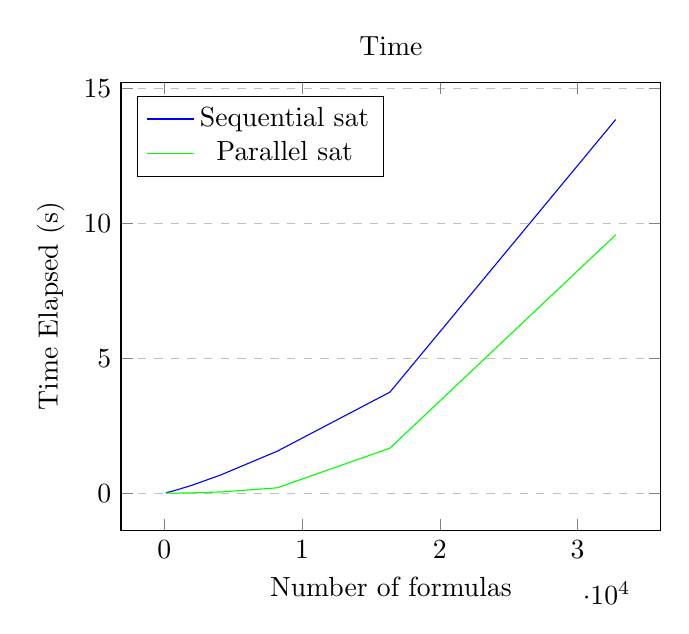
\begin{tikzpicture}
\begin{axis}[
title={Time},
ylabel={Time Elapsed (s)},
xlabel={Number of formulas},
legend pos=north west,
ymajorgrids=true,
grid style=dashed,
]

\addplot[color=blue]
coordinates {
	(128,0.0117)(256,0.0290)(512,0.0612)(1024,0.1374)(2048,0.2988)(4096,0.6736)(8192,1.5526)(16384,3.7465)(32768,13.8530)
};
\addplot[color=green]
coordinates {
	(128,0.0001)(256,0.0003)(512,0.0008)(1024,0.0026)(2048,0.0103)(4096,0.0442)(8192,0.1968)(16384,1.6690)(32768,9.5786)
};

\legend{Sequential sat,Parallel sat}

\end{axis}
\end{tikzpicture}

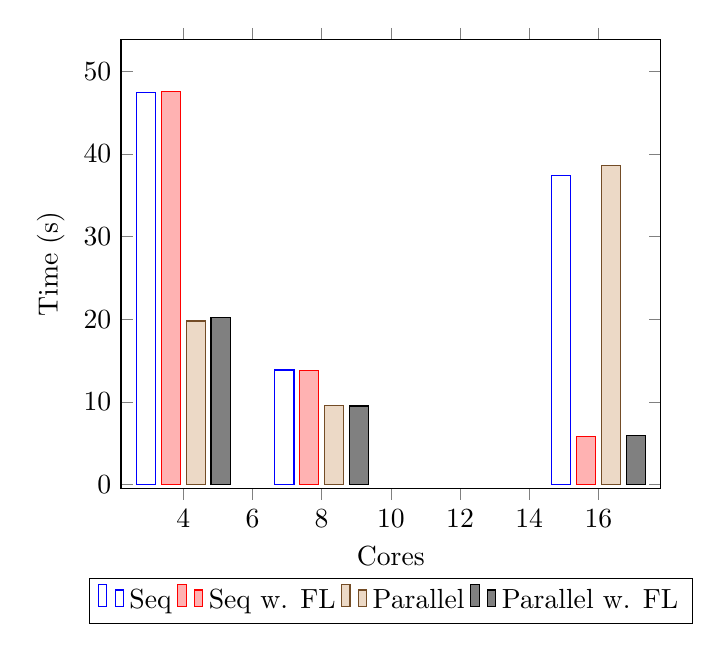
\begin{tikzpicture}
\begin{axis}[
x tick label style={
	/pgf/number format/1000 sep=},
ylabel=Time (s),
enlargelimits=0.15,
legend style={at={(0.5,-0.2)},
	anchor=north,legend columns=-1},
ybar,
bar width=7pt,
xlabel=Cores\\
]
\addplot[color=blue,domain=15:15]
coordinates {(4,47.4944)(8,13.8530)(16,37.3613)};
\addplot 
coordinates {(4,47.5747)(8,13.8145)(16,5.8145)};
\addplot 
coordinates {(4,19.7812)(8,9.5786)(16,38.5786)};
\addplot 
coordinates {(4,20.1922)(8,9.4844)(16,5.9145)};
\legend{Seq,Seq w. FL ,Parallel, Parallel w. FL}
\end{axis}
\end{tikzpicture}


\section{Conclusion}

\bibliography{biblio}
\bibliographystyle{ieeetr}


\appendix

\newpage
\newpage
% Please add the following required packages to your document preamble:
% \usepackage{booktabs}
% \usepackage{graphicx}
\begin{table}[htpb]
	\centering
	\caption{}
	\label{tab:my-table}
	\resizebox{\textwidth}{!}{%
		\begin{tabular}{@{}cclc@{}}
			\toprule
			\textbf{Theory} & \textbf{Source}   & \textbf{Formula}                                                                                           & \textbf{Result} \\ \midrule
			Equality        & Bradley-Manna     & f(x)=f(y)\&x!=y                                                                                            & SAT             \\
			&                   & x=y\&f(x)!=f(y)                                                                                            & UNSAT           \\
			&                   & f(a,b)=a\&f(f(a,b),b)!=a                                                                                   & UNSAT           \\
			&                   & f(f(f(a)))=a\&f(f(f(f(f(a)))))=a\&f(a)!=a                                                                  & UNSAT           \\
			&                   & f(f(f(a)))=f(f(a))\&f(f(f(f(a))))=a\&f(a)!=a                                                               & UNSAT           \\
			&                   & f(x,y)=f(y,x)\&f(a,y)!=f(y,a)                                                                              & SAT             \\
			&                   & f(g(x))=g(f(x))\&f(g(f(y)))=x\&f(y)=x\&g(f(x))!=x                                                          & UNSAT           \\
			& IC Tests          & b=d\&f(b)=d\&f(d)=a\&a!=b                                                                                  & UNSAT           \\
			&                   & a=b1\&b1=b2\&b2=b3\&b3=c\&f(a1,a1)=a\&f(c1,c1)=c\&a1=c1\&a!=c                                              & UNSAT           \\
			& Z3 Benchmark      & f1!=f2\&f3(f4,f5,f6,f7,f8(f9))!=f1\&f3(f4,f5,f6,f7,f10)=f1\&f10=f8(f9)\&f10=f8(f9)\&f3(f4,f5,f6,f7,f10)=f1 & UNSAT           \\
			&                   & f1!=f2\&f3(f4,f5,f6,f7,f8(f9))!=f1\&f3(f4,f5,f6,f7,f10)=f1\&f10=f8(f9)\&f3(f4,f5,f6,f7,f10)=f1             & UNSAT           \\
			&                   & f1!=f2\&f3(f4,f5,f6,f7,f8(f9))!=f1\&f3(f4,f5,f6,f7,f10)=f1\&f10=f8(f9)                                     & UNSAT           \\
			List            & Bradley Manna     & x1=x2\&y1=y2\&cons(x1,y1)!=cons(x2,y2)                                                                     & UNSAT           \\
			&                   & x=y\&car(x)!=car(y)                                                                                        & UNSAT           \\
			&                   & x=y\&cdr(x)!=cdr(y)                                                                                        & UNSAT           \\
			&                   & car(cons(x,y))!=x                                                                                          & UNSAT           \\
			&                   & cdr(cons(x,y))!=y                                                                                          & UNSAT           \\
			&                   & !atom(cons(x,y))                                                                                           & SAT             \\
			&                   & atom(x)\&cons(car(x),cdr(x))=x                                                                             & UNSAT           \\
			&                   & car(x)=car(y)\&cdr(x)=cdr(y)\&f(x)!=f(y)\&!atom(x)\&!atom(y)                                               & UNSAT           \\
			&                   & car(x)=y\&cdr(x)=z\&x!=cons(y,z)                                                                           & SAT             \\
			& Intermediate exam & f(b)=b\&f(f(b))!=car(cdr(cons(f(b),cons(b,d))))                                                            & UNSAT           \\
			Array           & Bradley-Manna     & i=k\&select(store(x,i,v),k)!=v                                                                             & UNSAT           \\
			&                   & i!=k\&select(store(x,i,v),k)!=select(x,k)                                                                  & UNSAT           \\
			&                   & i1=j\&i1!=i2\&select(a,j)=v1\&select(store(store(a,i1,v1),i2,v2),j)!=select(a,j)                           & UNSAT           \\
			& Intermediate exam & e=select(store(a,i,e),j)\&select(a,j)!=e                                                                   & SAT             \\ \bottomrule
		\end{tabular}%
	}
\end{table}
















\end{document}